\PassOptionsToPackage{unicode=true}{hyperref} % options for packages loaded elsewhere
\PassOptionsToPackage{hyphens}{url}
\PassOptionsToPackage{dvipsnames,svgnames*,x11names*}{xcolor}
%
\documentclass[]{article}
\usepackage{lmodern}
\usepackage{amssymb,amsmath}
\usepackage{ifxetex,ifluatex}
\usepackage{fixltx2e} % provides \textsubscript
\ifnum 0\ifxetex 1\fi\ifluatex 1\fi=0 % if pdftex
  \usepackage[T1]{fontenc}
  \usepackage[utf8]{inputenc}
  \usepackage{textcomp} % provides euro and other symbols
\else % if luatex or xelatex
  \usepackage{unicode-math}
  \defaultfontfeatures{Ligatures=TeX,Scale=MatchLowercase}
\fi
% use upquote if available, for straight quotes in verbatim environments
\IfFileExists{upquote.sty}{\usepackage{upquote}}{}
% use microtype if available
\IfFileExists{microtype.sty}{%
\usepackage[]{microtype}
\UseMicrotypeSet[protrusion]{basicmath} % disable protrusion for tt fonts
}{}
\IfFileExists{parskip.sty}{%
\usepackage{parskip}
}{% else
\setlength{\parindent}{0pt}
\setlength{\parskip}{6pt plus 2pt minus 1pt}
}
\usepackage{xcolor}
\usepackage{hyperref}
\hypersetup{
            pdfauthor={Nan Liu},
            colorlinks=true,
            linkcolor=Maroon,
            filecolor=Maroon,
            citecolor=Blue,
            urlcolor=blue,
            breaklinks=true}
\urlstyle{same}  % don't use monospace font for urls
\usepackage[margin=1in]{geometry}
\usepackage{color}
\usepackage{fancyvrb}
\newcommand{\VerbBar}{|}
\newcommand{\VERB}{\Verb[commandchars=\\\{\}]}
\DefineVerbatimEnvironment{Highlighting}{Verbatim}{commandchars=\\\{\}}
% Add ',fontsize=\small' for more characters per line
\usepackage{framed}
\definecolor{shadecolor}{RGB}{248,248,248}
\newenvironment{Shaded}{\begin{snugshade}}{\end{snugshade}}
\newcommand{\AlertTok}[1]{\textcolor[rgb]{0.94,0.16,0.16}{#1}}
\newcommand{\AnnotationTok}[1]{\textcolor[rgb]{0.56,0.35,0.01}{\textbf{\textit{#1}}}}
\newcommand{\AttributeTok}[1]{\textcolor[rgb]{0.77,0.63,0.00}{#1}}
\newcommand{\BaseNTok}[1]{\textcolor[rgb]{0.00,0.00,0.81}{#1}}
\newcommand{\BuiltInTok}[1]{#1}
\newcommand{\CharTok}[1]{\textcolor[rgb]{0.31,0.60,0.02}{#1}}
\newcommand{\CommentTok}[1]{\textcolor[rgb]{0.56,0.35,0.01}{\textit{#1}}}
\newcommand{\CommentVarTok}[1]{\textcolor[rgb]{0.56,0.35,0.01}{\textbf{\textit{#1}}}}
\newcommand{\ConstantTok}[1]{\textcolor[rgb]{0.00,0.00,0.00}{#1}}
\newcommand{\ControlFlowTok}[1]{\textcolor[rgb]{0.13,0.29,0.53}{\textbf{#1}}}
\newcommand{\DataTypeTok}[1]{\textcolor[rgb]{0.13,0.29,0.53}{#1}}
\newcommand{\DecValTok}[1]{\textcolor[rgb]{0.00,0.00,0.81}{#1}}
\newcommand{\DocumentationTok}[1]{\textcolor[rgb]{0.56,0.35,0.01}{\textbf{\textit{#1}}}}
\newcommand{\ErrorTok}[1]{\textcolor[rgb]{0.64,0.00,0.00}{\textbf{#1}}}
\newcommand{\ExtensionTok}[1]{#1}
\newcommand{\FloatTok}[1]{\textcolor[rgb]{0.00,0.00,0.81}{#1}}
\newcommand{\FunctionTok}[1]{\textcolor[rgb]{0.00,0.00,0.00}{#1}}
\newcommand{\ImportTok}[1]{#1}
\newcommand{\InformationTok}[1]{\textcolor[rgb]{0.56,0.35,0.01}{\textbf{\textit{#1}}}}
\newcommand{\KeywordTok}[1]{\textcolor[rgb]{0.13,0.29,0.53}{\textbf{#1}}}
\newcommand{\NormalTok}[1]{#1}
\newcommand{\OperatorTok}[1]{\textcolor[rgb]{0.81,0.36,0.00}{\textbf{#1}}}
\newcommand{\OtherTok}[1]{\textcolor[rgb]{0.56,0.35,0.01}{#1}}
\newcommand{\PreprocessorTok}[1]{\textcolor[rgb]{0.56,0.35,0.01}{\textit{#1}}}
\newcommand{\RegionMarkerTok}[1]{#1}
\newcommand{\SpecialCharTok}[1]{\textcolor[rgb]{0.00,0.00,0.00}{#1}}
\newcommand{\SpecialStringTok}[1]{\textcolor[rgb]{0.31,0.60,0.02}{#1}}
\newcommand{\StringTok}[1]{\textcolor[rgb]{0.31,0.60,0.02}{#1}}
\newcommand{\VariableTok}[1]{\textcolor[rgb]{0.00,0.00,0.00}{#1}}
\newcommand{\VerbatimStringTok}[1]{\textcolor[rgb]{0.31,0.60,0.02}{#1}}
\newcommand{\WarningTok}[1]{\textcolor[rgb]{0.56,0.35,0.01}{\textbf{\textit{#1}}}}
\usepackage{graphicx,grffile}
\makeatletter
\def\maxwidth{\ifdim\Gin@nat@width>\linewidth\linewidth\else\Gin@nat@width\fi}
\def\maxheight{\ifdim\Gin@nat@height>\textheight\textheight\else\Gin@nat@height\fi}
\makeatother
% Scale images if necessary, so that they will not overflow the page
% margins by default, and it is still possible to overwrite the defaults
% using explicit options in \includegraphics[width, height, ...]{}
\setkeys{Gin}{width=\maxwidth,height=\maxheight,keepaspectratio}
\setlength{\emergencystretch}{3em}  % prevent overfull lines
\providecommand{\tightlist}{%
  \setlength{\itemsep}{0pt}\setlength{\parskip}{0pt}}
\setcounter{secnumdepth}{0}
% Redefines (sub)paragraphs to behave more like sections
\ifx\paragraph\undefined\else
\let\oldparagraph\paragraph
\renewcommand{\paragraph}[1]{\oldparagraph{#1}\mbox{}}
\fi
\ifx\subparagraph\undefined\else
\let\oldsubparagraph\subparagraph
\renewcommand{\subparagraph}[1]{\oldsubparagraph{#1}\mbox{}}
\fi

% set default figure placement to htbp
\makeatletter
\def\fps@figure{htbp}
\makeatother

\usepackage{amsgen,amsmath,amstext,amsbsy,amsopn,amssymb,mathabx,amsthm,bm,bbm}
\usepackage{etoolbox}
\makeatletter
\providecommand{\subtitle}[1]{% add subtitle to \maketitle
  \apptocmd{\@title}{\par {\large #1 \par}}{}{}
}
\makeatother

\title{\textbf {BIOSTAT 285 Spring 2020 Homework 2}}
\providecommand{\subtitle}[1]{}
\subtitle{\textbf{Due by 11:00 PM, 05/14/2020}}
\author{Nan Liu}
\date{}

\begin{document}
\maketitle

\theoremstyle{definition}
\newtheorem*{hint}{Hint}

\theoremstyle{remark}
\newtheorem*{rmk}{Remark}

\emph{Remark.} For \textbf{Computational Part}, please complete your
answer in the \textbf{RMarkdown} file and summit the generated PDF and
RMD files.

\hypertarget{computational-part}{%
\subsection{Computational Part}\label{computational-part}}

\begin{enumerate}
\def\labelenumi{\arabic{enumi}.}
\tightlist
\item
  ({[}ISL{]} 4.11, \emph{25 pt}) In this problem, you will develop a
  model to predict whether a given car gets high or low gas mileage
  based on the \texttt{Auto} data set. Write a data analysis report
  addressing the following problems.
\end{enumerate}

\begin{enumerate}
\def\labelenumi{(\alph{enumi})}
\tightlist
\item
  Create a binary variable, \texttt{mpg01}, that contains a 1 if
  \texttt{mpg} contains a value above its median, and a 0 if
  \texttt{mpg} contains a value below its median.
\end{enumerate}

\begin{Shaded}
\begin{Highlighting}[]
\KeywordTok{library}\NormalTok{(ISLR) }
\KeywordTok{data}\NormalTok{(}\StringTok{"Auto"}\NormalTok{) }
\end{Highlighting}
\end{Shaded}

\begin{Shaded}
\begin{Highlighting}[]
\KeywordTok{set.seed}\NormalTok{(}\DecValTok{123}\NormalTok{)}
\NormalTok{Auto <-}\StringTok{ }\NormalTok{Auto }\OperatorTok
\StringTok{  }\KeywordTok{mutate}\NormalTok{ (}\DataTypeTok{mpg01 =} \KeywordTok{factor}\NormalTok{(}\KeywordTok{ifelse}\NormalTok{(mpg }\OperatorTok{>}\StringTok{ }\KeywordTok{median}\NormalTok{(mpg), }\DecValTok{1}\NormalTok{, }\DecValTok{0}\NormalTok{)))}
\KeywordTok{median}\NormalTok{(Auto}\OperatorTok{$}\NormalTok{mpg)}
\end{Highlighting}
\end{Shaded}

\begin{verbatim}
## [1] 22.75
\end{verbatim}

\begin{enumerate}
\def\labelenumi{(\alph{enumi})}
\setcounter{enumi}{1}
\tightlist
\item
  Explore the data graphically in order to investigate the association
  between \texttt{mgp01} and the other features. Which of the other
  features seem most likely to be useful in predicting \texttt{mpg01}?
  Scatterplots and boxplots may be useful tools to answer this question.
  Describe your findings.
\end{enumerate}

\begin{Shaded}
\begin{Highlighting}[]
\CommentTok{#scatter plots}
\KeywordTok{pairs}\NormalTok{(Auto)}
\end{Highlighting}
\end{Shaded}

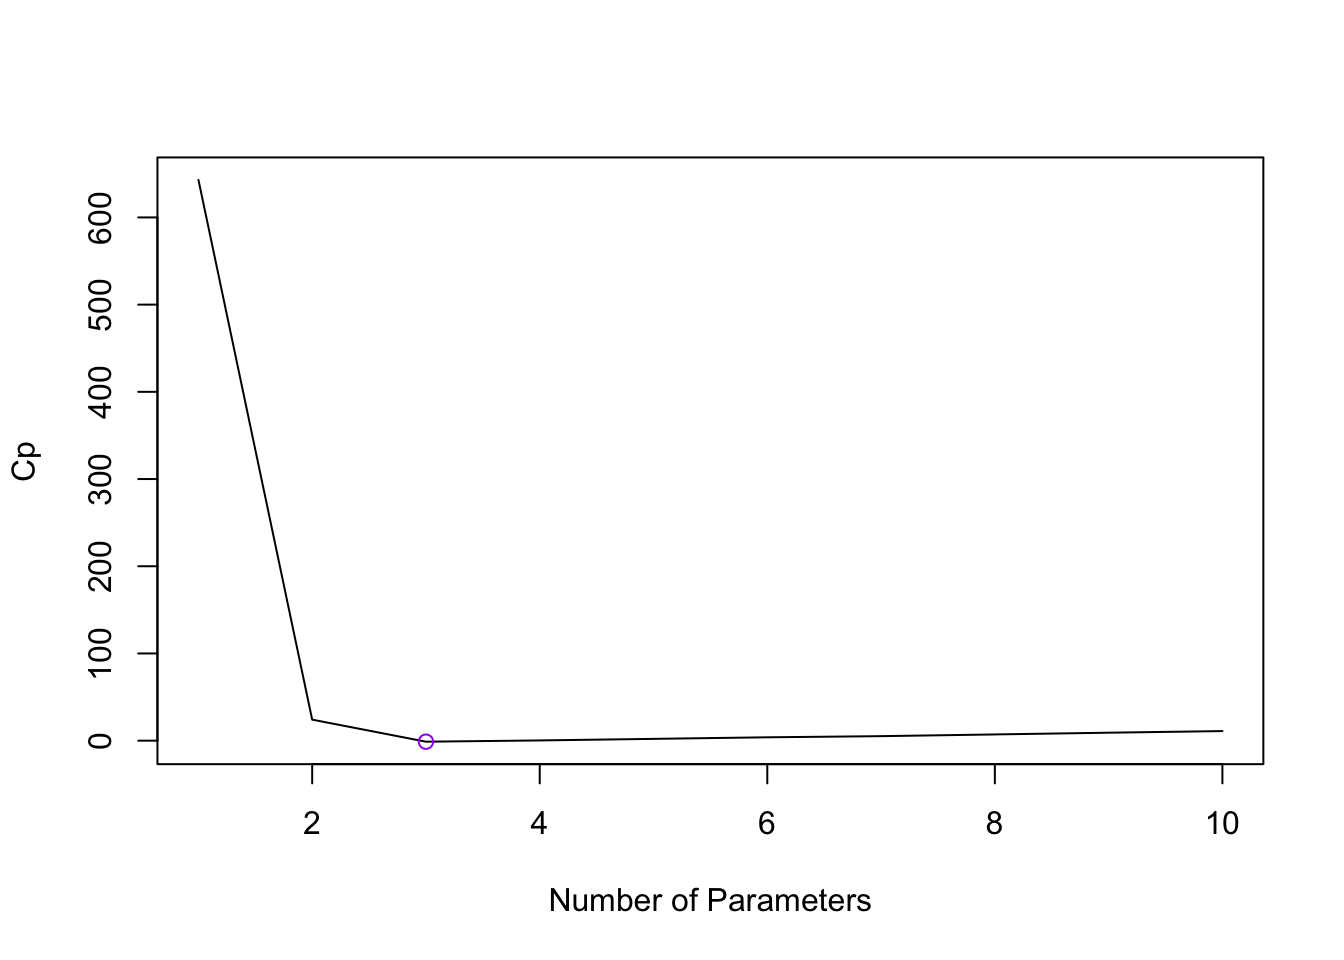
\includegraphics{hw2compsol_files/figure-latex/unnamed-chunk-4-1.pdf}

From the scatter plot, we assume `cylinders', `displacement',
`horsepower' and `weight' seem mostly likely to be useful in predicting
\texttt{mpg01}.

\newpage

Now let's display the boxplot

\begin{Shaded}
\begin{Highlighting}[]
\CommentTok{#Boxplots}
\KeywordTok{ggplot}\NormalTok{(Auto, }\KeywordTok{aes}\NormalTok{(mpg01,cylinders)) }\OperatorTok{+}\StringTok{ }\KeywordTok{geom_boxplot}\NormalTok{()}
\end{Highlighting}
\end{Shaded}

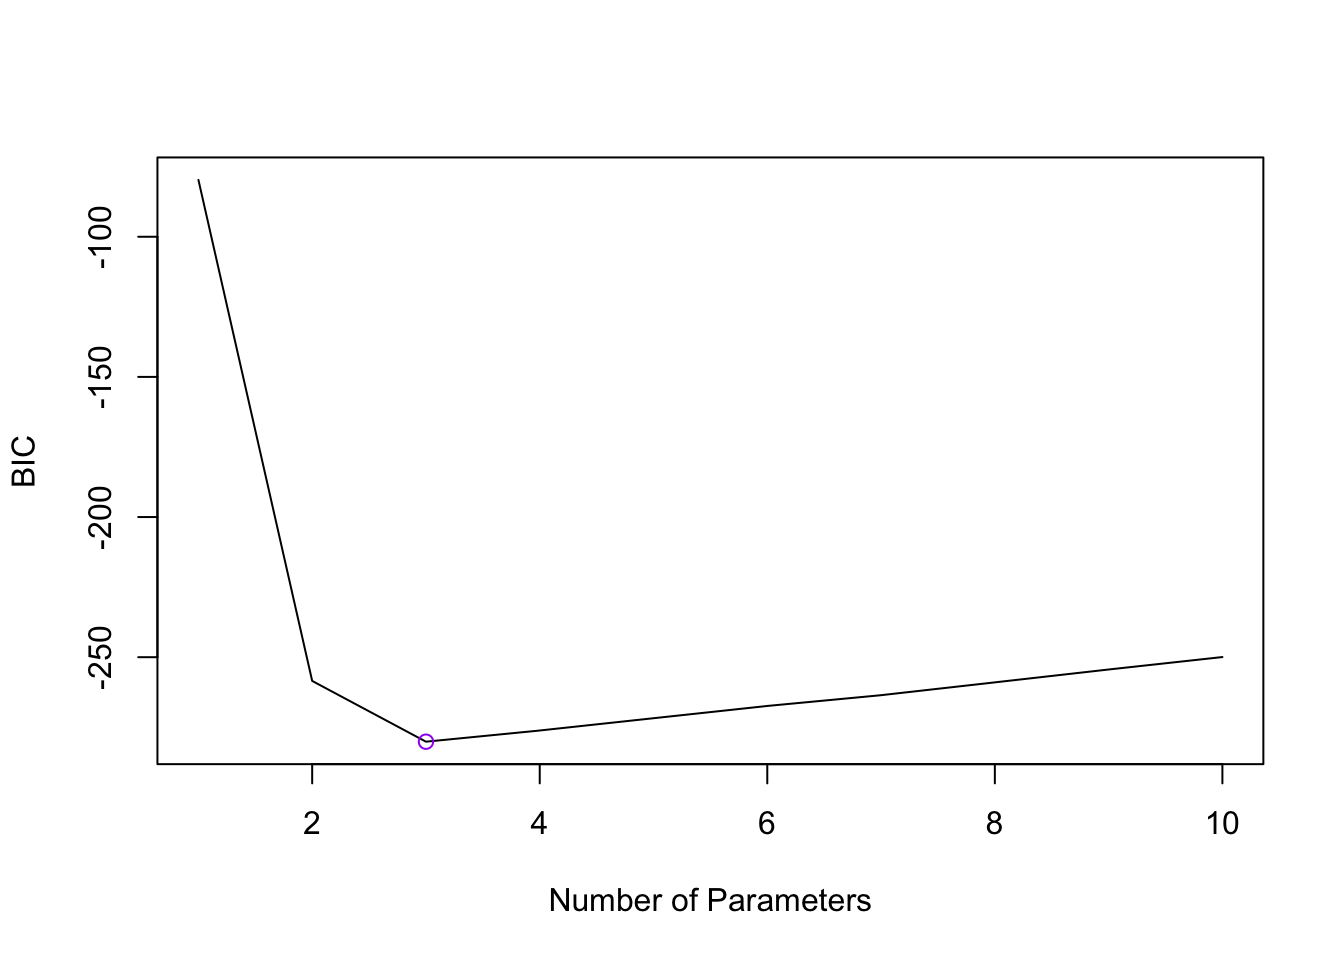
\includegraphics{hw2compsol_files/figure-latex/unnamed-chunk-5-1.pdf}
\newpage

\begin{Shaded}
\begin{Highlighting}[]
\KeywordTok{ggplot}\NormalTok{(Auto, }\KeywordTok{aes}\NormalTok{(mpg01,displacement)) }\OperatorTok{+}\StringTok{ }\KeywordTok{geom_boxplot}\NormalTok{()}
\end{Highlighting}
\end{Shaded}

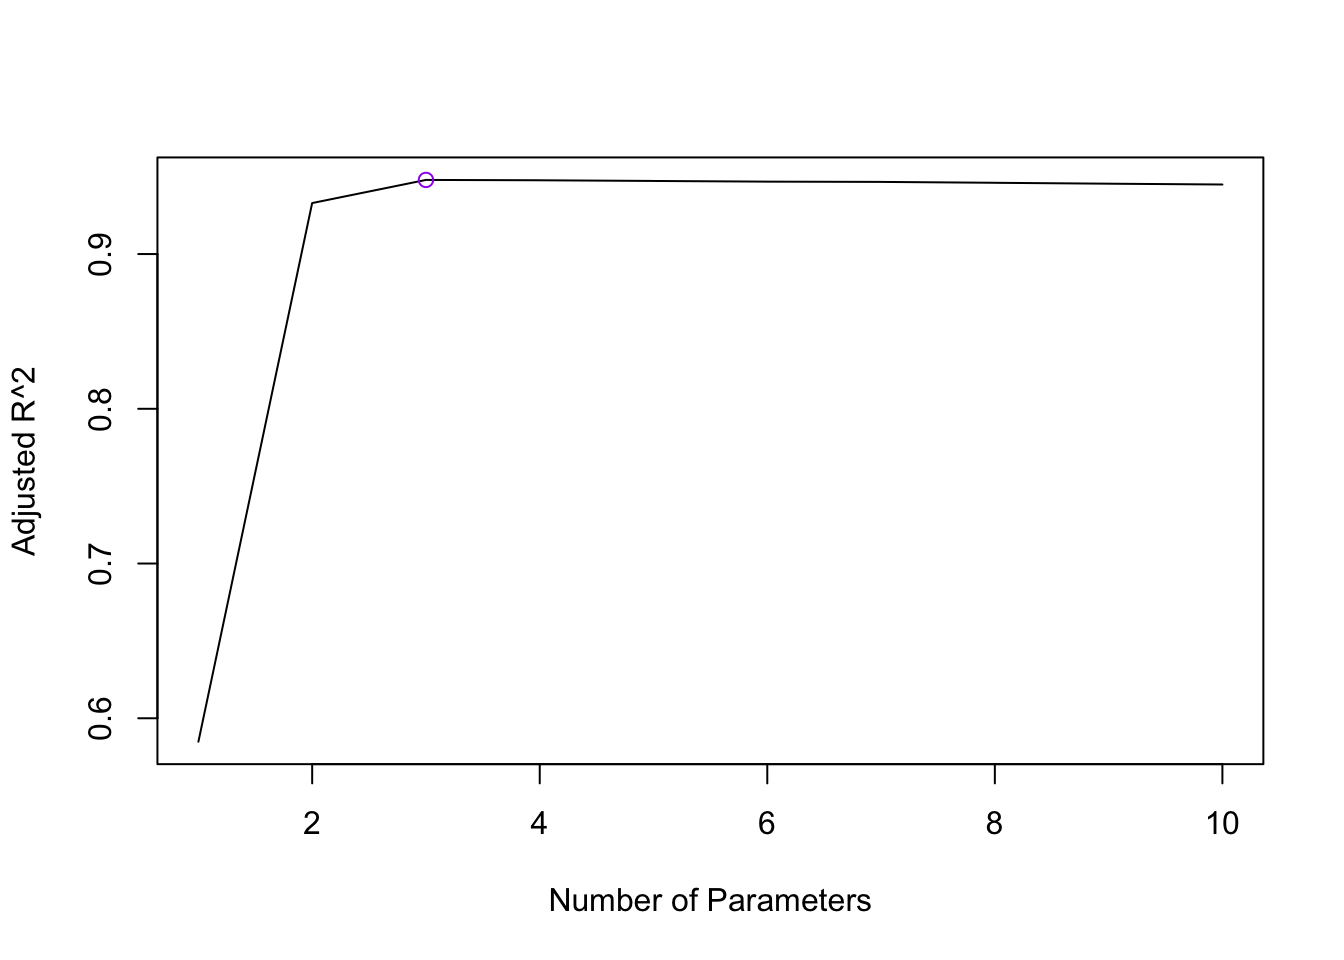
\includegraphics{hw2compsol_files/figure-latex/unnamed-chunk-6-1.pdf}
\newpage

\begin{Shaded}
\begin{Highlighting}[]
\KeywordTok{ggplot}\NormalTok{(Auto, }\KeywordTok{aes}\NormalTok{(mpg01, horsepower)) }\OperatorTok{+}\StringTok{ }\KeywordTok{geom_boxplot}\NormalTok{()}
\end{Highlighting}
\end{Shaded}

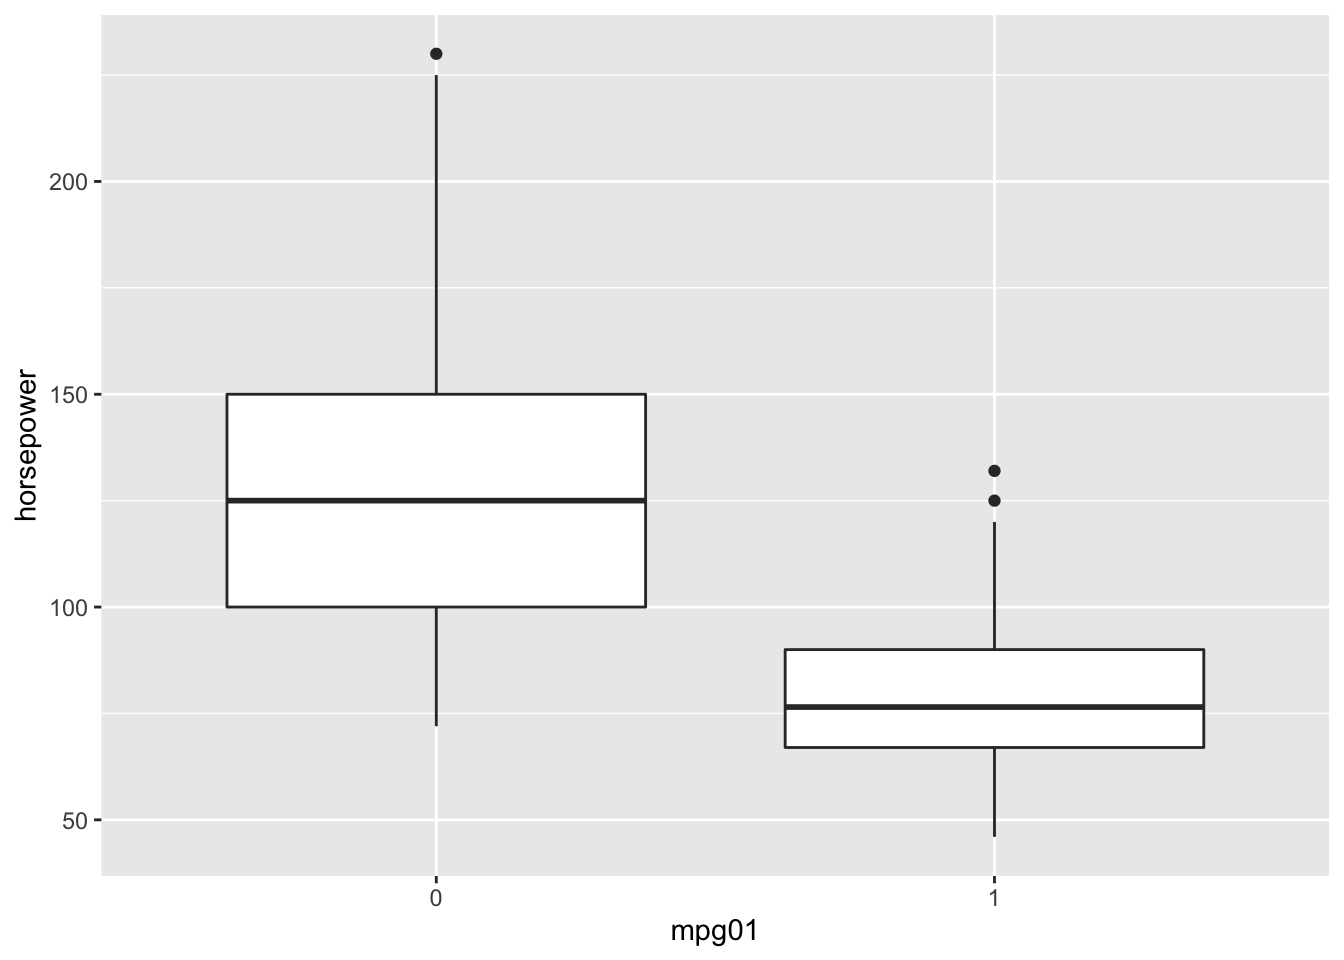
\includegraphics{hw2compsol_files/figure-latex/unnamed-chunk-7-1.pdf}
\newpage

\begin{Shaded}
\begin{Highlighting}[]
\KeywordTok{ggplot}\NormalTok{(Auto, }\KeywordTok{aes}\NormalTok{(mpg01,weight)) }\OperatorTok{+}\StringTok{ }\KeywordTok{geom_boxplot}\NormalTok{()}
\end{Highlighting}
\end{Shaded}

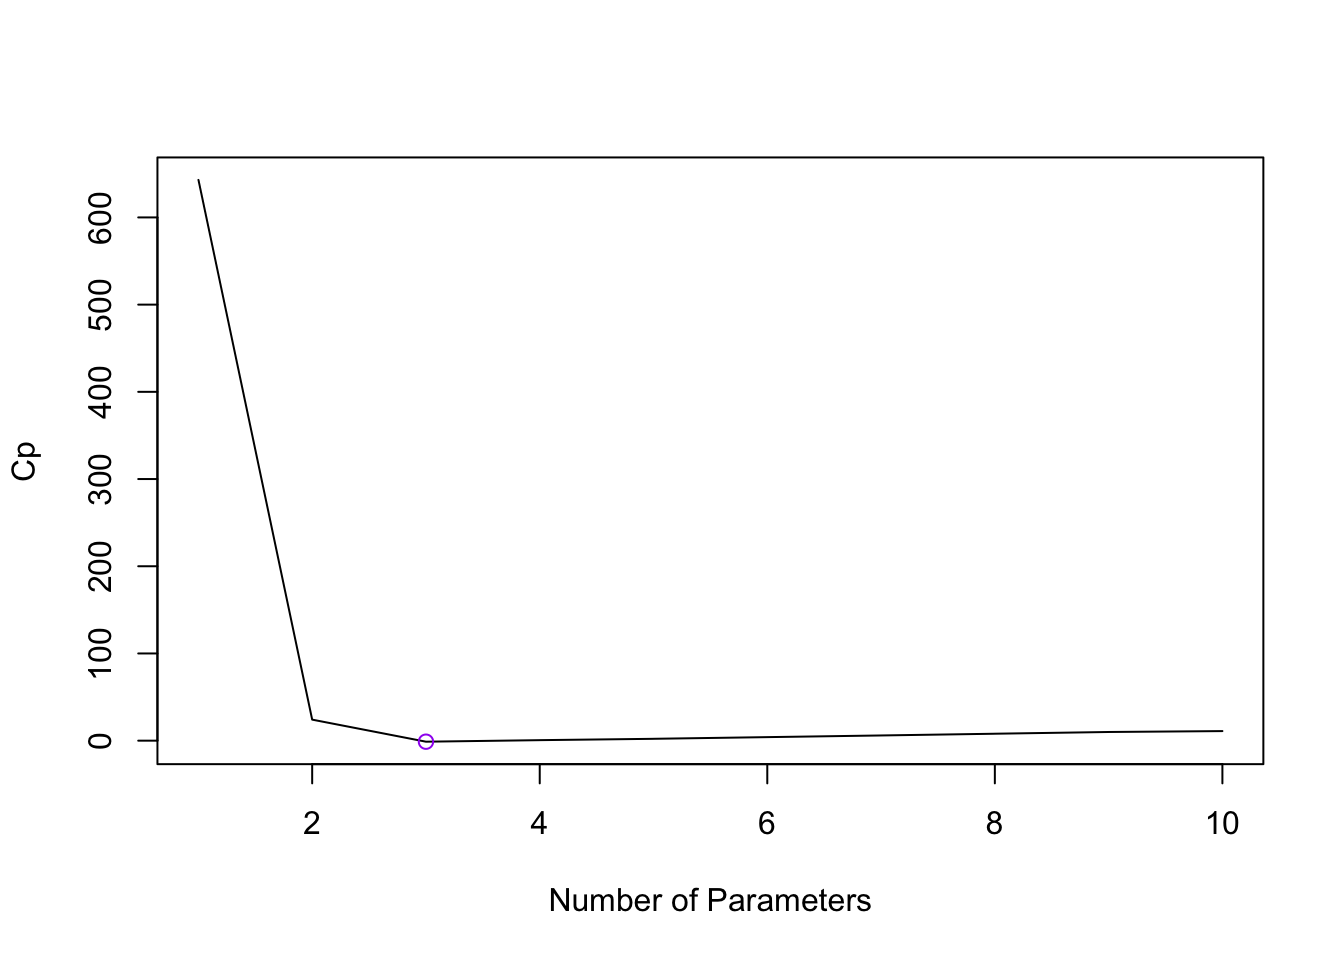
\includegraphics{hw2compsol_files/figure-latex/unnamed-chunk-8-1.pdf}

\begin{enumerate}
\def\labelenumi{(\alph{enumi})}
\setcounter{enumi}{2}
\tightlist
\item
  Split the data into a training set and a test set.
\end{enumerate}

\begin{Shaded}
\begin{Highlighting}[]
\CommentTok{#split data in to 70% traing set and 30% test set}
\KeywordTok{set.seed}\NormalTok{(}\DecValTok{123}\NormalTok{)}
\NormalTok{s <-}\StringTok{ }\KeywordTok{sample}\NormalTok{(}\KeywordTok{nrow}\NormalTok{(Auto), }\KeywordTok{floor}\NormalTok{(}\KeywordTok{nrow}\NormalTok{(Auto)}\OperatorTok{*}\FloatTok{0.7}\NormalTok{), }\DataTypeTok{replace =}\NormalTok{ F)}
\NormalTok{training <-}\StringTok{ }\NormalTok{Auto[s,]}
\NormalTok{test <-}\StringTok{ }\NormalTok{Auto[}\OperatorTok{-}\NormalTok{s,]}
\end{Highlighting}
\end{Shaded}

\begin{enumerate}
\def\labelenumi{(\alph{enumi})}
\setcounter{enumi}{3}
\tightlist
\item
  Perform LDA on the training data in order to predict \texttt{mpg01}
  using the variables that seemed most associated with \texttt{mpg01} in
  (b). What is the test error of the model obtained?
\end{enumerate}

\begin{Shaded}
\begin{Highlighting}[]
\KeywordTok{library}\NormalTok{(MASS)}
\end{Highlighting}
\end{Shaded}

\begin{verbatim}
## Warning: package 'MASS' was built under R version 3.6.2
\end{verbatim}

\begin{verbatim}
## 
## Attaching package: 'MASS'
\end{verbatim}

\begin{verbatim}
## The following object is masked from 'package:dplyr':
## 
##     select
\end{verbatim}

\begin{Shaded}
\begin{Highlighting}[]
\NormalTok{lda.fit <-}\StringTok{ }\KeywordTok{lda}\NormalTok{(mpg01 }\OperatorTok{~}\StringTok{ }\NormalTok{cylinders }\OperatorTok{+}\StringTok{ }\NormalTok{displacement }\OperatorTok{+}\StringTok{ }\NormalTok{horsepower }\OperatorTok{+}\StringTok{ }\NormalTok{weight, }\DataTypeTok{data =}\NormalTok{ training)}

\CommentTok{#test error}
\NormalTok{lda.pred <-}\StringTok{ }\KeywordTok{predict}\NormalTok{(lda.fit, test)}
\KeywordTok{mean}\NormalTok{(lda.pred}\OperatorTok{$}\NormalTok{class }\OperatorTok{!=}\StringTok{ }\NormalTok{test}\OperatorTok{$}\NormalTok{mpg01)}
\end{Highlighting}
\end{Shaded}

\begin{verbatim}
## [1] 0.1101695
\end{verbatim}

The test error is about 11\%.

\begin{enumerate}
\def\labelenumi{(\alph{enumi})}
\setcounter{enumi}{4}
\tightlist
\item
  Perform QDA on the training data in order to predict \texttt{mpg01}
  using the variables that seemed most associated with \texttt{mpg01} in
  (b). What is the test error of the model obtained?
\end{enumerate}

\begin{Shaded}
\begin{Highlighting}[]
\NormalTok{qda.fit <-}\StringTok{ }\KeywordTok{qda}\NormalTok{(mpg01 }\OperatorTok{~}\StringTok{ }\NormalTok{cylinders }\OperatorTok{+}\StringTok{ }\NormalTok{displacement }\OperatorTok{+}\StringTok{ }\NormalTok{horsepower }\OperatorTok{+}\StringTok{ }\NormalTok{weight, }\DataTypeTok{data =}\NormalTok{ training)}

\CommentTok{#test error}
\NormalTok{qda.class <-}\StringTok{ }\KeywordTok{predict}\NormalTok{(qda.fit, test)}\OperatorTok{$}\NormalTok{class}
\KeywordTok{mean}\NormalTok{(qda.class }\OperatorTok{!=}\StringTok{ }\NormalTok{test}\OperatorTok{$}\NormalTok{mpg01)}
\end{Highlighting}
\end{Shaded}

\begin{verbatim}
## [1] 0.1016949
\end{verbatim}

The test error is about 10\%

\begin{enumerate}
\def\labelenumi{(\alph{enumi})}
\setcounter{enumi}{5}
\tightlist
\item
  Perform logistic regression on the training data in order to predict
  \texttt{mpg01} using the variables that seemed most associated with
  \texttt{mpg01} in (b). What is the test error of the model obtained?
\end{enumerate}

\begin{Shaded}
\begin{Highlighting}[]
\NormalTok{glm.fit <-}\StringTok{ }\KeywordTok{glm}\NormalTok{(mpg01 }\OperatorTok{~}\StringTok{ }\NormalTok{cylinders }\OperatorTok{+}\StringTok{ }\NormalTok{displacement }\OperatorTok{+}\StringTok{ }\NormalTok{horsepower }\OperatorTok{+}\StringTok{ }\NormalTok{weight, }
               \DataTypeTok{data =}\NormalTok{ training, }\DataTypeTok{family=}\NormalTok{binomial)}
\CommentTok{#test error}
\NormalTok{prob <-}\StringTok{ }\KeywordTok{predict}\NormalTok{(glm.fit, test, }\DataTypeTok{type =} \StringTok{"response"}\NormalTok{)}
\NormalTok{glm.pred <-}\StringTok{ }\KeywordTok{ifelse}\NormalTok{(prob }\OperatorTok{>}\StringTok{ }\FloatTok{0.5}\NormalTok{, }\DecValTok{1}\NormalTok{, }\DecValTok{0}\NormalTok{)}
\KeywordTok{mean}\NormalTok{(glm.pred }\OperatorTok{!=}\StringTok{ }\NormalTok{test}\OperatorTok{$}\NormalTok{mpg01)}
\end{Highlighting}
\end{Shaded}

\begin{verbatim}
## [1] 0.1101695
\end{verbatim}

The test error is about 11\%

\textbf{Report}

From the scatter plot, we assume `cylinders', `displacement',
`horsepower' and `weight' seem mostly likely to be useful in predicting
\texttt{mpg01}. The box plots also agree with this variable selection.
Then we split our data into 70\% traing set and 30\% test set. In order
to predict \texttt{mpg01}, we perform LDA, QDA and logistic regression
on the training set using the variables `cylinders', `displacement',
`horsepower' and `weight'. The test error from LDA method, QDA method
and logistic regression method are all about 11\%.

\begin{enumerate}
\def\labelenumi{\arabic{enumi}.}
\setcounter{enumi}{1}
\tightlist
\item
  (New York Times Covid-19 State Data, \emph{35 pt}) Download the data
  file \texttt{covid-19-state-level-data.csv}, then answer the following
  questions using splines.
\end{enumerate}

\begin{enumerate}
\def\labelenumi{(\alph{enumi})}
\tightlist
\item
  Create subsets of the data for States New York, California, and
  Washington. Print out the dimension and first 6 observations of each
  state subset.
\end{enumerate}

\begin{Shaded}
\begin{Highlighting}[]
\CommentTok{#import csv file}
\NormalTok{covid <-}\StringTok{ }\KeywordTok{read.csv}\NormalTok{(}\StringTok{"covid-19-state-level-data.csv"}\NormalTok{)}
\CommentTok{#subset new york}
\NormalTok{ny <-}\StringTok{ }\KeywordTok{filter}\NormalTok{(covid, state }\OperatorTok{==}\StringTok{ "New York"}\NormalTok{)}
\KeywordTok{dim}\NormalTok{(ny)}
\end{Highlighting}
\end{Shaded}

\begin{verbatim}
## [1] 58  5
\end{verbatim}

\begin{Shaded}
\begin{Highlighting}[]
\KeywordTok{head}\NormalTok{(ny,}\DecValTok{6}\NormalTok{)}
\end{Highlighting}
\end{Shaded}

\begin{verbatim}
##         date    state fips cases deaths
## 1 2020-03-01 New York   36     1      0
## 2 2020-03-02 New York   36     1      0
## 3 2020-03-03 New York   36     2      0
## 4 2020-03-04 New York   36    11      0
## 5 2020-03-05 New York   36    22      0
## 6 2020-03-06 New York   36    44      0
\end{verbatim}

\begin{Shaded}
\begin{Highlighting}[]
\CommentTok{#california}
\NormalTok{ca <-}\StringTok{ }\KeywordTok{filter}\NormalTok{(covid, state }\OperatorTok{==}\StringTok{ "California"}\NormalTok{) }
\KeywordTok{dim}\NormalTok{(ca)}
\end{Highlighting}
\end{Shaded}

\begin{verbatim}
## [1] 94  5
\end{verbatim}

\begin{Shaded}
\begin{Highlighting}[]
\KeywordTok{head}\NormalTok{(ca,}\DecValTok{6}\NormalTok{)}
\end{Highlighting}
\end{Shaded}

\begin{verbatim}
##         date      state fips cases deaths
## 1 2020-01-25 California    6     1      0
## 2 2020-01-26 California    6     2      0
## 3 2020-01-27 California    6     2      0
## 4 2020-01-28 California    6     2      0
## 5 2020-01-29 California    6     2      0
## 6 2020-01-30 California    6     2      0
\end{verbatim}

\begin{Shaded}
\begin{Highlighting}[]
\CommentTok{#washington}
\NormalTok{wa <-}\StringTok{ }\KeywordTok{filter}\NormalTok{(covid, state }\OperatorTok{==}\StringTok{ "Washington"}\NormalTok{) }
\KeywordTok{dim}\NormalTok{(wa)}
\end{Highlighting}
\end{Shaded}

\begin{verbatim}
## [1] 98  5
\end{verbatim}

\begin{Shaded}
\begin{Highlighting}[]
\KeywordTok{head}\NormalTok{(wa,}\DecValTok{6}\NormalTok{)}
\end{Highlighting}
\end{Shaded}

\begin{verbatim}
##         date      state fips cases deaths
## 1 2020-01-21 Washington   53     1      0
## 2 2020-01-22 Washington   53     1      0
## 3 2020-01-23 Washington   53     1      0
## 4 2020-01-24 Washington   53     1      0
## 5 2020-01-25 Washington   53     1      0
## 6 2020-01-26 Washington   53     1      0
\end{verbatim}

\begin{enumerate}
\def\labelenumi{(\alph{enumi})}
\setcounter{enumi}{1}
\tightlist
\item
  Fit both cubic splines (using \texttt{bs}) and natural cubic splines
  (using \texttt{ns}) on each subset, with the number of cases as
  response, and the number of days since first case as predictor. Find
  the optimal degrees of freedom (\texttt{df}) for the basis.
\end{enumerate}

\begin{Shaded}
\begin{Highlighting}[]
\CommentTok{#generate the number of days since first case}
\NormalTok{ny <-}\StringTok{ }\NormalTok{ny }\OperatorTok
\StringTok{  }\KeywordTok{mutate}\NormalTok{(}\DataTypeTok{days =} \KeywordTok{as.numeric}\NormalTok{(}\KeywordTok{as.Date}\NormalTok{(}\KeywordTok{as.character}\NormalTok{(date))}\OperatorTok{-}
\StringTok{                  }\KeywordTok{as.Date}\NormalTok{(}\KeywordTok{as.character}\NormalTok{(}\StringTok{"2020-03-01"}\NormalTok{))))}
\NormalTok{ca <-}\StringTok{ }\NormalTok{ca }\OperatorTok
\StringTok{  }\KeywordTok{mutate}\NormalTok{(}\DataTypeTok{days =} \KeywordTok{as.numeric}\NormalTok{(}\KeywordTok{as.Date}\NormalTok{(}\KeywordTok{as.character}\NormalTok{(date))}\OperatorTok{-}
\StringTok{                  }\KeywordTok{as.Date}\NormalTok{(}\KeywordTok{as.character}\NormalTok{(}\StringTok{"2020-01-25"}\NormalTok{))))}
\NormalTok{wa <-}\StringTok{ }\NormalTok{wa }\OperatorTok
\StringTok{  }\KeywordTok{mutate}\NormalTok{(}\DataTypeTok{days =} \KeywordTok{as.numeric}\NormalTok{(}\KeywordTok{as.Date}\NormalTok{(}\KeywordTok{as.character}\NormalTok{(date))}\OperatorTok{-}
\StringTok{                  }\KeywordTok{as.Date}\NormalTok{(}\KeywordTok{as.character}\NormalTok{(}\StringTok{"2020-01-21"}\NormalTok{))))}
\end{Highlighting}
\end{Shaded}

\begin{Shaded}
\begin{Highlighting}[]
\CommentTok{#find the optimal degree of freedom}
\CommentTok{#split 80% training, 20% test}
\KeywordTok{set.seed}\NormalTok{(}\DecValTok{6}\NormalTok{)}
\NormalTok{s <-}\StringTok{ }\KeywordTok{sample}\NormalTok{(}\KeywordTok{nrow}\NormalTok{(ny), }\KeywordTok{floor}\NormalTok{(}\KeywordTok{nrow}\NormalTok{(ny)}\OperatorTok{*}\FloatTok{0.8}\NormalTok{), }\DataTypeTok{replace =}\NormalTok{ F)}
\NormalTok{nytraining <-}\StringTok{ }\NormalTok{ny[s,]}
\NormalTok{nytest <-}\StringTok{ }\NormalTok{ny[}\OperatorTok{-}\NormalTok{s,]}

\KeywordTok{library}\NormalTok{(splines)}
\CommentTok{#bs }
\NormalTok{se <-}\StringTok{ }\KeywordTok{c}\NormalTok{()}
\ControlFlowTok{for}\NormalTok{ (i }\ControlFlowTok{in} \DecValTok{3}\OperatorTok{:}\DecValTok{40}\NormalTok{)\{}
\NormalTok{fit <-}\StringTok{ }\KeywordTok{lm}\NormalTok{(cases }\OperatorTok{~}\StringTok{ }\KeywordTok{bs}\NormalTok{(days, }\DataTypeTok{df =}\NormalTok{ i, }\DataTypeTok{knots =} \OtherTok{NULL}\NormalTok{, }
                       \DataTypeTok{degree =} \DecValTok{3}\NormalTok{, }\DataTypeTok{intercept =} \OtherTok{FALSE}\NormalTok{), }\DataTypeTok{data =}\NormalTok{ nytraining)}
\NormalTok{pred <-}\StringTok{ }\KeywordTok{predict}\NormalTok{(fit, nytest)}
\NormalTok{se[i] <-}\StringTok{ }\KeywordTok{mean}\NormalTok{((pred }\OperatorTok{-}\StringTok{ }\NormalTok{nytest}\OperatorTok{$}\NormalTok{cases)}\OperatorTok{^}\DecValTok{2}\NormalTok{)}
\NormalTok{\}}
\KeywordTok{which.min}\NormalTok{(se)}
\end{Highlighting}
\end{Shaded}

\begin{verbatim}
## [1] 39
\end{verbatim}

\begin{Shaded}
\begin{Highlighting}[]
\CommentTok{#ns }
\NormalTok{se <-}\StringTok{ }\KeywordTok{c}\NormalTok{()}
\ControlFlowTok{for}\NormalTok{ (i }\ControlFlowTok{in} \DecValTok{3}\OperatorTok{:}\DecValTok{40}\NormalTok{)\{}
\NormalTok{fit <-}\StringTok{ }\KeywordTok{lm}\NormalTok{(cases }\OperatorTok{~}\StringTok{ }\KeywordTok{ns}\NormalTok{(days, }\DataTypeTok{df =}\NormalTok{ i, }\DataTypeTok{knots =} \OtherTok{NULL}\NormalTok{, }
                     \DataTypeTok{intercept =} \OtherTok{FALSE}\NormalTok{), }\DataTypeTok{data =}\NormalTok{ nytraining)}
\NormalTok{pred <-}\StringTok{ }\KeywordTok{predict}\NormalTok{(fit, nytest) }
\NormalTok{se[i] <-}\StringTok{ }\KeywordTok{mean}\NormalTok{((pred }\OperatorTok{-}\StringTok{ }\NormalTok{nytest}\OperatorTok{$}\NormalTok{cases)}\OperatorTok{^}\DecValTok{2}\NormalTok{)}
\NormalTok{\}}
\KeywordTok{which.min}\NormalTok{(se)}
\end{Highlighting}
\end{Shaded}

\begin{verbatim}
## [1] 37
\end{verbatim}

The optimal degree of freedom for New York is 39 when using cubic
splines and 37 when using natural cubic splines.

\begin{Shaded}
\begin{Highlighting}[]
\CommentTok{#split 80% training, 20% test}
\KeywordTok{set.seed}\NormalTok{(}\DecValTok{8}\NormalTok{)}
\NormalTok{s <-}\StringTok{ }\KeywordTok{sample}\NormalTok{(}\KeywordTok{nrow}\NormalTok{(ca), }\KeywordTok{floor}\NormalTok{(}\KeywordTok{nrow}\NormalTok{(ca)}\OperatorTok{*}\FloatTok{0.8}\NormalTok{), }\DataTypeTok{replace =}\NormalTok{ F)}
\NormalTok{catraining <-}\StringTok{ }\NormalTok{ca[s,]}
\NormalTok{catest <-}\StringTok{ }\NormalTok{ca[}\OperatorTok{-}\NormalTok{s,]}

\CommentTok{#bs df = 37}
\NormalTok{se <-}\StringTok{ }\KeywordTok{c}\NormalTok{()}
\ControlFlowTok{for}\NormalTok{ (i }\ControlFlowTok{in} \DecValTok{3}\OperatorTok{:}\DecValTok{40}\NormalTok{)\{}
\NormalTok{fit <-}\StringTok{ }\KeywordTok{lm}\NormalTok{(cases }\OperatorTok{~}\StringTok{ }\KeywordTok{bs}\NormalTok{(days, }\DataTypeTok{df =}\NormalTok{ i, }\DataTypeTok{knots =} \OtherTok{NULL}\NormalTok{, }\DataTypeTok{degree =} \DecValTok{3}\NormalTok{, }
                     \DataTypeTok{intercept =} \OtherTok{FALSE}\NormalTok{), }\DataTypeTok{data =}\NormalTok{ catraining)}
\NormalTok{pred <-}\StringTok{ }\KeywordTok{predict}\NormalTok{(fit, catest)}
\NormalTok{se[i] <-}\StringTok{ }\KeywordTok{mean}\NormalTok{((pred }\OperatorTok{-}\StringTok{ }\NormalTok{catest}\OperatorTok{$}\NormalTok{cases)}\OperatorTok{^}\DecValTok{2}\NormalTok{)}
\NormalTok{\}}
\KeywordTok{which.min}\NormalTok{(se)}
\end{Highlighting}
\end{Shaded}

\begin{verbatim}
## [1] 37
\end{verbatim}

\begin{Shaded}
\begin{Highlighting}[]
\CommentTok{#ns df = 29}
\NormalTok{se <-}\StringTok{ }\KeywordTok{c}\NormalTok{()}
\ControlFlowTok{for}\NormalTok{ (i }\ControlFlowTok{in} \DecValTok{3}\OperatorTok{:}\DecValTok{40}\NormalTok{)\{}
\NormalTok{fit <-}\StringTok{ }\KeywordTok{lm}\NormalTok{(cases }\OperatorTok{~}\StringTok{ }\KeywordTok{ns}\NormalTok{(days, }\DataTypeTok{df =}\NormalTok{ i, }\DataTypeTok{knots =} \OtherTok{NULL}\NormalTok{, }
                     \DataTypeTok{intercept =} \OtherTok{FALSE}\NormalTok{), }\DataTypeTok{data =}\NormalTok{ catraining)}
\NormalTok{pred <-}\StringTok{ }\KeywordTok{predict}\NormalTok{(fit, catest) }
\NormalTok{se[i] <-}\StringTok{ }\KeywordTok{mean}\NormalTok{((pred }\OperatorTok{-}\StringTok{ }\NormalTok{catest}\OperatorTok{$}\NormalTok{cases)}\OperatorTok{^}\DecValTok{2}\NormalTok{)}
\NormalTok{\}}
\KeywordTok{which.min}\NormalTok{(se)}
\end{Highlighting}
\end{Shaded}

\begin{verbatim}
## [1] 29
\end{verbatim}

The optimal degree of freedom for California is 37 when using cubic
splines and 29 when using natural cubic splines.

\begin{Shaded}
\begin{Highlighting}[]
\CommentTok{#split 80% training, 20% test}
\KeywordTok{set.seed}\NormalTok{(}\DecValTok{8}\NormalTok{)}
\NormalTok{s <-}\StringTok{ }\KeywordTok{sample}\NormalTok{(}\KeywordTok{nrow}\NormalTok{(wa), }\KeywordTok{floor}\NormalTok{(}\KeywordTok{nrow}\NormalTok{(wa)}\OperatorTok{*}\FloatTok{0.8}\NormalTok{), }\DataTypeTok{replace =}\NormalTok{ F)}
\NormalTok{watraining <-}\StringTok{ }\NormalTok{wa[s,]}
\NormalTok{watest <-}\StringTok{ }\NormalTok{wa[}\OperatorTok{-}\NormalTok{s,]}

\CommentTok{#bs df = 38}
\NormalTok{se <-}\StringTok{ }\KeywordTok{c}\NormalTok{()}
\ControlFlowTok{for}\NormalTok{ (i }\ControlFlowTok{in} \DecValTok{3}\OperatorTok{:}\DecValTok{40}\NormalTok{)\{}
\NormalTok{fit <-}\StringTok{ }\KeywordTok{lm}\NormalTok{(cases }\OperatorTok{~}\StringTok{ }\KeywordTok{bs}\NormalTok{(days, }\DataTypeTok{df =}\NormalTok{ i, }\DataTypeTok{knots =} \OtherTok{NULL}\NormalTok{, }\DataTypeTok{degree =} \DecValTok{3}\NormalTok{,}
                     \DataTypeTok{intercept =} \OtherTok{FALSE}\NormalTok{), }\DataTypeTok{data =}\NormalTok{ watraining)}
\NormalTok{pred <-}\StringTok{ }\KeywordTok{predict}\NormalTok{(fit, watest)}
\NormalTok{se[i] <-}\StringTok{ }\KeywordTok{mean}\NormalTok{((pred }\OperatorTok{-}\StringTok{ }\NormalTok{watest}\OperatorTok{$}\NormalTok{cases)}\OperatorTok{^}\DecValTok{2}\NormalTok{)}
\NormalTok{\}}
\KeywordTok{which.min}\NormalTok{(se)}
\end{Highlighting}
\end{Shaded}

\begin{verbatim}
## [1] 38
\end{verbatim}

\begin{Shaded}
\begin{Highlighting}[]
\CommentTok{#ns df = 36}
\NormalTok{se <-}\StringTok{ }\KeywordTok{c}\NormalTok{()}
\ControlFlowTok{for}\NormalTok{ (i }\ControlFlowTok{in} \DecValTok{3}\OperatorTok{:}\DecValTok{40}\NormalTok{)\{}
\NormalTok{fit <-}\StringTok{ }\KeywordTok{lm}\NormalTok{(cases }\OperatorTok{~}\StringTok{ }\KeywordTok{ns}\NormalTok{(days, }\DataTypeTok{df =}\NormalTok{ i, }\DataTypeTok{knots =} \OtherTok{NULL}\NormalTok{, }
                     \DataTypeTok{intercept =} \OtherTok{FALSE}\NormalTok{), }\DataTypeTok{data =}\NormalTok{ watraining)}
\NormalTok{pred <-}\StringTok{ }\KeywordTok{predict}\NormalTok{(fit, watest) }
\NormalTok{se[i] <-}\StringTok{ }\KeywordTok{mean}\NormalTok{((pred }\OperatorTok{-}\StringTok{ }\NormalTok{watest}\OperatorTok{$}\NormalTok{cases)}\OperatorTok{^}\DecValTok{2}\NormalTok{)}
\NormalTok{\}}
\KeywordTok{which.min}\NormalTok{(se)}
\end{Highlighting}
\end{Shaded}

\begin{verbatim}
## [1] 36
\end{verbatim}

The optimal degree of freedom for Washington is 38 when using cubic
splines and 36 when using natural cubic splines.

\begin{Shaded}
\begin{Highlighting}[]
\CommentTok{#ny}
\NormalTok{ny.bs <-}\StringTok{ }\KeywordTok{bs}\NormalTok{(ny}\OperatorTok{$}\NormalTok{days, }\DataTypeTok{df =} \DecValTok{39}\NormalTok{, }\DataTypeTok{knots =} \OtherTok{NULL}\NormalTok{, }
            \DataTypeTok{degree =} \DecValTok{3}\NormalTok{, }\DataTypeTok{intercept =} \OtherTok{FALSE}\NormalTok{) }
\NormalTok{ny.ns <-}\StringTok{ }\KeywordTok{ns}\NormalTok{(ny}\OperatorTok{$}\NormalTok{days, }\DataTypeTok{df =} \DecValTok{37}\NormalTok{, }\DataTypeTok{knots =} \OtherTok{NULL}\NormalTok{, }
            \DataTypeTok{intercept =} \OtherTok{FALSE}\NormalTok{)}
\CommentTok{#ca}
\NormalTok{ca.bs <-}\StringTok{ }\KeywordTok{bs}\NormalTok{(ca}\OperatorTok{$}\NormalTok{days, }\DataTypeTok{df =} \DecValTok{37}\NormalTok{, }\DataTypeTok{knots =} \OtherTok{NULL}\NormalTok{, }
            \DataTypeTok{degree =} \DecValTok{3}\NormalTok{, }\DataTypeTok{intercept =} \OtherTok{FALSE}\NormalTok{)}
\NormalTok{ca.ns <-}\StringTok{ }\KeywordTok{ns}\NormalTok{(ca}\OperatorTok{$}\NormalTok{days, }\DataTypeTok{df =} \DecValTok{29}\NormalTok{, }\DataTypeTok{knots =} \OtherTok{NULL}\NormalTok{,}
            \DataTypeTok{intercept =} \OtherTok{FALSE}\NormalTok{)}
\CommentTok{#washington}
\NormalTok{wa.bs <-}\StringTok{ }\KeywordTok{bs}\NormalTok{(wa}\OperatorTok{$}\NormalTok{days, }\DataTypeTok{df =} \DecValTok{38}\NormalTok{, }\DataTypeTok{knots =} \OtherTok{NULL}\NormalTok{, }
            \DataTypeTok{degree =} \DecValTok{3}\NormalTok{, }\DataTypeTok{intercept =} \OtherTok{FALSE}\NormalTok{)}
\NormalTok{wa.ns <-}\StringTok{ }\KeywordTok{ns}\NormalTok{(wa}\OperatorTok{$}\NormalTok{days, }\DataTypeTok{df =} \DecValTok{36}\NormalTok{, }\DataTypeTok{knots =} \OtherTok{NULL}\NormalTok{, }
            \DataTypeTok{intercept =} \OtherTok{FALSE}\NormalTok{)}
\end{Highlighting}
\end{Shaded}

\begin{enumerate}
\def\labelenumi{(\alph{enumi})}
\setcounter{enumi}{2}
\tightlist
\item
  Generate a plot of three panels, each corresponding to one state. Each
  panel plots the observed data and the fitted splines (different colors
  for cubic spline and NCS). Compare and commment on the two types of
  splines.
\end{enumerate}

\begin{Shaded}
\begin{Highlighting}[]
\NormalTok{ny.bs.fit <-}\StringTok{ }\KeywordTok{lm}\NormalTok{(cases }\OperatorTok{~}\StringTok{ }\KeywordTok{bs}\NormalTok{(days, }\DataTypeTok{df =} \DecValTok{39}\NormalTok{, }\DataTypeTok{knots =} \OtherTok{NULL}\NormalTok{, }\DataTypeTok{degree =} \DecValTok{3}\NormalTok{), }\DataTypeTok{data =}\NormalTok{ ny)}
\NormalTok{prednybs <-}\StringTok{ }\KeywordTok{predict}\NormalTok{(ny.bs.fit,}\DataTypeTok{data =}\NormalTok{ ny)}


\NormalTok{ny.ns.fit <-}\StringTok{ }\KeywordTok{lm}\NormalTok{(cases }\OperatorTok{~}\StringTok{ }\KeywordTok{ns}\NormalTok{(days, }\DataTypeTok{df =} \DecValTok{37}\NormalTok{, }\DataTypeTok{knots =} \OtherTok{NULL}\NormalTok{, }
            \DataTypeTok{intercept =} \OtherTok{FALSE}\NormalTok{), }\DataTypeTok{data =}\NormalTok{ ny)}
\NormalTok{prednyns <-}\StringTok{ }\KeywordTok{predict}\NormalTok{(ny.ns.fit, }\DataTypeTok{data =}\NormalTok{ ny)}
\end{Highlighting}
\end{Shaded}

\begin{Shaded}
\begin{Highlighting}[]
\KeywordTok{plot}\NormalTok{(ny}\OperatorTok{$}\NormalTok{days,ny}\OperatorTok{$}\NormalTok{cases, }\DataTypeTok{type =} \StringTok{"o"}\NormalTok{,}
     \DataTypeTok{xlab =} \StringTok{"days"}\NormalTok{,}
     \DataTypeTok{ylab =} \StringTok{"cases"}\NormalTok{,}
     \DataTypeTok{col =} \StringTok{"gray"}\NormalTok{)}
\KeywordTok{lines}\NormalTok{(ny}\OperatorTok{$}\NormalTok{days,prednyns, }\DataTypeTok{type =} \StringTok{"l"}\NormalTok{,}
     \DataTypeTok{xlab =} \StringTok{"days"}\NormalTok{,}
     \DataTypeTok{ylab =} \StringTok{"cases"}\NormalTok{, }
     \DataTypeTok{col =} \StringTok{"dark red"}\NormalTok{)}
\KeywordTok{lines}\NormalTok{(ny}\OperatorTok{$}\NormalTok{days,prednybs, }\DataTypeTok{xlab =} \OtherTok{NULL}\NormalTok{, }\DataTypeTok{ylab =} \OtherTok{NULL}\NormalTok{, }
      \DataTypeTok{lty =} \DecValTok{2}\NormalTok{, }\DataTypeTok{type =} \StringTok{"l"}\NormalTok{,}\DataTypeTok{col =} \StringTok{"green"}\NormalTok{, }\KeywordTok{title}\NormalTok{(}\StringTok{"New York"}\NormalTok{))}
\KeywordTok{legend}\NormalTok{(}\DecValTok{0}\NormalTok{,}\DecValTok{200000}\NormalTok{,}\DataTypeTok{legend=}\KeywordTok{c}\NormalTok{(}\StringTok{"observed data"}\NormalTok{,}\StringTok{"nature spline"}\NormalTok{,}\StringTok{"cubic spline"}\NormalTok{), }
       \DataTypeTok{col=}\KeywordTok{c}\NormalTok{(}\StringTok{"gray"}\NormalTok{,}\StringTok{"dark red"}\NormalTok{,}\StringTok{"green"}\NormalTok{), }\DataTypeTok{pch =} \KeywordTok{c}\NormalTok{(}\DecValTok{1}\NormalTok{, }\OtherTok{NA}\NormalTok{, }\OtherTok{NA}\NormalTok{),}
        \DataTypeTok{lty=}\KeywordTok{c}\NormalTok{(}\OtherTok{NA}\NormalTok{,}\DecValTok{1}\NormalTok{,}\DecValTok{2}\NormalTok{), }\DataTypeTok{ncol=}\DecValTok{1}\NormalTok{)}
\end{Highlighting}
\end{Shaded}

\includegraphics{hw2compsol_files/figure-latex/unnamed-chunk-25-1.pdf}

\begin{Shaded}
\begin{Highlighting}[]
\CommentTok{#new form nearly the same}
\NormalTok{ca.bs.fit <-}\StringTok{ }\KeywordTok{lm}\NormalTok{(cases }\OperatorTok{~}\StringTok{ }\KeywordTok{bs}\NormalTok{(days, }\DataTypeTok{df =} \DecValTok{37}\NormalTok{, }\DataTypeTok{knots =} \OtherTok{NULL}\NormalTok{, }
            \DataTypeTok{degree =} \DecValTok{3}\NormalTok{, }\DataTypeTok{intercept =} \OtherTok{FALSE}\NormalTok{), }\DataTypeTok{data =}\NormalTok{ ca)}
\NormalTok{predcabs <-}\StringTok{ }\KeywordTok{predict}\NormalTok{(ca.bs.fit,}\DataTypeTok{data =}\NormalTok{ ca)}
\NormalTok{ca.ns.fit <-}\StringTok{ }\KeywordTok{lm}\NormalTok{(cases }\OperatorTok{~}\StringTok{ }\KeywordTok{ns}\NormalTok{(days, }\DataTypeTok{df =} \DecValTok{29}\NormalTok{, }\DataTypeTok{knots =} \OtherTok{NULL}\NormalTok{,}
            \DataTypeTok{intercept =} \OtherTok{FALSE}\NormalTok{), }\DataTypeTok{data =}\NormalTok{ ca)}
\NormalTok{predcans <-}\StringTok{ }\KeywordTok{predict}\NormalTok{(ca.ns.fit, }\DataTypeTok{data =}\NormalTok{ ca)}
\KeywordTok{plot}\NormalTok{(ca}\OperatorTok{$}\NormalTok{days,ca}\OperatorTok{$}\NormalTok{cases, }\DataTypeTok{type =} \StringTok{"o"}\NormalTok{,}
     \DataTypeTok{xlab =} \StringTok{"days"}\NormalTok{,}
     \DataTypeTok{ylab =} \StringTok{"cases"}\NormalTok{,}
     \DataTypeTok{col =} \StringTok{"gray"}\NormalTok{)}
\KeywordTok{lines}\NormalTok{(ca}\OperatorTok{$}\NormalTok{days,predcans, }\DataTypeTok{type =} \StringTok{"l"}\NormalTok{,}
     \DataTypeTok{xlab =} \StringTok{"days"}\NormalTok{,}
     \DataTypeTok{ylab =} \StringTok{"cases"}\NormalTok{, }
     \DataTypeTok{col =} \StringTok{"dark red"}\NormalTok{)}
\KeywordTok{lines}\NormalTok{(ca}\OperatorTok{$}\NormalTok{days,predcabs, }\DataTypeTok{xlab =} \OtherTok{NULL}\NormalTok{, }\DataTypeTok{ylab =} \OtherTok{NULL}\NormalTok{, }
      \DataTypeTok{lty =} \DecValTok{2}\NormalTok{, }\DataTypeTok{type =} \StringTok{"l"}\NormalTok{,}\DataTypeTok{col =} \StringTok{"green"}\NormalTok{, }\KeywordTok{title}\NormalTok{(}\StringTok{"California"}\NormalTok{))}
\KeywordTok{legend}\NormalTok{(}\DecValTok{0}\NormalTok{,}\DecValTok{30000}\NormalTok{,}\DataTypeTok{legend=}\KeywordTok{c}\NormalTok{(}\StringTok{"observed data"}\NormalTok{,}\StringTok{"nature spline"}\NormalTok{,}\StringTok{"cubic spline"}\NormalTok{), }
       \DataTypeTok{col=}\KeywordTok{c}\NormalTok{(}\StringTok{"gray"}\NormalTok{,}\StringTok{"dark red"}\NormalTok{,}\StringTok{"green"}\NormalTok{), }\DataTypeTok{pch =} \KeywordTok{c}\NormalTok{(}\DecValTok{1}\NormalTok{,}\OtherTok{NA}\NormalTok{, }\OtherTok{NA}\NormalTok{),}
        \DataTypeTok{lty=}\KeywordTok{c}\NormalTok{(}\OtherTok{NA}\NormalTok{, }\DecValTok{1}\NormalTok{,}\DecValTok{2}\NormalTok{), }\DataTypeTok{ncol=}\DecValTok{1}\NormalTok{)}
\end{Highlighting}
\end{Shaded}

\includegraphics{hw2compsol_files/figure-latex/unnamed-chunk-26-1.pdf}

\begin{Shaded}
\begin{Highlighting}[]
\NormalTok{wa.bs.fit <-}\StringTok{ }\KeywordTok{lm}\NormalTok{(cases }\OperatorTok{~}\StringTok{ }\KeywordTok{bs}\NormalTok{(days, }\DataTypeTok{knots =} \OtherTok{NULL}\NormalTok{, }\DataTypeTok{df =} \DecValTok{38}\NormalTok{, }
                           \DataTypeTok{degree =} \DecValTok{3}\NormalTok{, }\DataTypeTok{intercept =} \OtherTok{FALSE}\NormalTok{), }\DataTypeTok{data =}\NormalTok{ wa)}
\NormalTok{predwabs <-}\StringTok{ }\KeywordTok{predict}\NormalTok{(wa.bs.fit,}\DataTypeTok{data =}\NormalTok{ wa)}
\NormalTok{wa.ns.fit <-}\StringTok{ }\KeywordTok{lm}\NormalTok{(cases }\OperatorTok{~}\StringTok{ }\KeywordTok{ns}\NormalTok{(days, }\DataTypeTok{df =} \DecValTok{36}\NormalTok{, }\DataTypeTok{knots =} \OtherTok{NULL}\NormalTok{, }
            \DataTypeTok{intercept =} \OtherTok{FALSE}\NormalTok{), }\DataTypeTok{data =}\NormalTok{ wa)}
\NormalTok{predwans <-}\StringTok{ }\KeywordTok{predict}\NormalTok{(wa.ns.fit, }\DataTypeTok{data =}\NormalTok{ wa)}
\end{Highlighting}
\end{Shaded}

\begin{Shaded}
\begin{Highlighting}[]
\KeywordTok{plot}\NormalTok{(wa}\OperatorTok{$}\NormalTok{days,wa}\OperatorTok{$}\NormalTok{cases, }\DataTypeTok{type =} \StringTok{"o"}\NormalTok{,}
     \DataTypeTok{xlab =} \StringTok{"days"}\NormalTok{,}
     \DataTypeTok{ylab =} \StringTok{"cases"}\NormalTok{,}
     \DataTypeTok{col =} \StringTok{"gray"}\NormalTok{)}
\KeywordTok{lines}\NormalTok{(wa}\OperatorTok{$}\NormalTok{days,predwans, }\DataTypeTok{type =} \StringTok{"l"}\NormalTok{,}
     \DataTypeTok{xlab =} \StringTok{"days"}\NormalTok{,}
     \DataTypeTok{ylab =} \StringTok{"cases"}\NormalTok{, }
     \DataTypeTok{col =} \StringTok{"dark red"}\NormalTok{)}
\KeywordTok{lines}\NormalTok{(wa}\OperatorTok{$}\NormalTok{days,predwabs, }\DataTypeTok{xlab =} \OtherTok{NULL}\NormalTok{, }\DataTypeTok{ylab =} \OtherTok{NULL}\NormalTok{, }
      \DataTypeTok{lty =} \DecValTok{2}\NormalTok{, }\DataTypeTok{type =} \StringTok{"l"}\NormalTok{,}\DataTypeTok{col =} \StringTok{"green"}\NormalTok{, }\KeywordTok{title}\NormalTok{(}\StringTok{"Washington"}\NormalTok{))}
\KeywordTok{legend}\NormalTok{(}\DecValTok{0}\NormalTok{,}\DecValTok{8000}\NormalTok{,}\DataTypeTok{legend=}\KeywordTok{c}\NormalTok{(}\StringTok{"observed data"}\NormalTok{,}\StringTok{"nature spline"}\NormalTok{,}\StringTok{"cubic spline"}\NormalTok{), }
       \DataTypeTok{col=}\KeywordTok{c}\NormalTok{(}\StringTok{"gray"}\NormalTok{,}\StringTok{"dark red"}\NormalTok{,}\StringTok{"green"}\NormalTok{), }\DataTypeTok{pch =} \KeywordTok{c}\NormalTok{(}\DecValTok{1}\NormalTok{,}\OtherTok{NA}\NormalTok{, }\OtherTok{NA}\NormalTok{),}
        \DataTypeTok{lty=}\KeywordTok{c}\NormalTok{(}\OtherTok{NA}\NormalTok{,}\DecValTok{1}\NormalTok{,}\DecValTok{2}\NormalTok{), }\DataTypeTok{ncol=}\DecValTok{1}\NormalTok{)}
\end{Highlighting}
\end{Shaded}

\includegraphics{hw2compsol_files/figure-latex/unnamed-chunk-28-1.pdf}

If we specify the degree of freedom to be the optimal degree of freedom,
the two lines nearly coincide. The cubic splines and natural cubic
splines result in similar fitted values on these three subsets. From the
plot we know the cubic splines and natural cubic splines can both
describe the model pretty well on the 3 subsets.

\begin{enumerate}
\def\labelenumi{(\alph{enumi})}
\setcounter{enumi}{3}
\tightlist
\item
  Use the fitted splines from Washington and California to predict the
  number of cases in New York State. Which prediction is better? Comment
  on why/why not the prediction is good.
\end{enumerate}

\begin{Shaded}
\begin{Highlighting}[]
\CommentTok{#washington bs}
\NormalTok{predwabs <-}\StringTok{ }\KeywordTok{predict}\NormalTok{(wa.bs.fit, ny)}
\KeywordTok{mean}\NormalTok{((predwabs }\OperatorTok{-}\StringTok{ }\NormalTok{ny}\OperatorTok{$}\NormalTok{cases)}\OperatorTok{^}\DecValTok{2}\NormalTok{)}
\end{Highlighting}
\end{Shaded}

\begin{verbatim}
## [1] 20334956650
\end{verbatim}

\begin{Shaded}
\begin{Highlighting}[]
\CommentTok{#washington ns}
\NormalTok{predwans <-}\StringTok{ }\KeywordTok{predict}\NormalTok{(wa.ns.fit, ny)}
\KeywordTok{mean}\NormalTok{((predwans }\OperatorTok{-}\StringTok{ }\NormalTok{ny}\OperatorTok{$}\NormalTok{cases)}\OperatorTok{^}\DecValTok{2}\NormalTok{)}
\end{Highlighting}
\end{Shaded}

\begin{verbatim}
## [1] 20334956635
\end{verbatim}

\begin{Shaded}
\begin{Highlighting}[]
\CommentTok{#ca bs}
\NormalTok{predcabs <-}\StringTok{ }\KeywordTok{predict}\NormalTok{(ca.bs.fit, }\DataTypeTok{newdata =}\NormalTok{ ny)}
\KeywordTok{mean}\NormalTok{((predcabs }\OperatorTok{-}\StringTok{ }\NormalTok{ny}\OperatorTok{$}\NormalTok{cases)}\OperatorTok{^}\DecValTok{2}\NormalTok{)}
\end{Highlighting}
\end{Shaded}

\begin{verbatim}
## [1] 20297165754
\end{verbatim}

\begin{Shaded}
\begin{Highlighting}[]
\CommentTok{#ca ns}
\NormalTok{predcans<-}\StringTok{ }\KeywordTok{predict}\NormalTok{(ca.ns.fit, }\DataTypeTok{newdata =}\NormalTok{ ny)}
\KeywordTok{mean}\NormalTok{((predcans }\OperatorTok{-}\StringTok{ }\NormalTok{ny}\OperatorTok{$}\NormalTok{cases)}\OperatorTok{^}\DecValTok{2}\NormalTok{)}
\end{Highlighting}
\end{Shaded}

\begin{verbatim}
## [1] 20297826747
\end{verbatim}

Both cubic splines and natural cubic splines result in quite large and
similar test error. The predictions are not good because New York has
far more cases than those in California and Washington. Also, the growth
rate of cases in New York is much higher than those of the other 2
states.

\begin{enumerate}
\def\labelenumi{(\alph{enumi})}
\setcounter{enumi}{4}
\tightlist
\item
  Now use Smoothing Spline (\texttt{smooth.spline}) to fit the
  California data, and predict its number of cases in the next 30 days.
  Plot the observed data, the fitted line, and its extrapolation in a
  single plot. Comment on the prediction you get.
\end{enumerate}

\begin{Shaded}
\begin{Highlighting}[]
\CommentTok{## develop a model}
\NormalTok{smooth.fit <-}\StringTok{ }\KeywordTok{smooth.spline}\NormalTok{(}\DataTypeTok{x =}\NormalTok{ca[,}\StringTok{"days"}\NormalTok{], }
                            \DataTypeTok{y =}\NormalTok{ ca[,}\StringTok{"cases"}\NormalTok{], }\DataTypeTok{w =} \OtherTok{NULL}\NormalTok{, }\DataTypeTok{cv =} \OtherTok{FALSE}\NormalTok{)}
\NormalTok{cafit <-}\StringTok{ }\KeywordTok{data.frame}\NormalTok{(}\DataTypeTok{days =}\NormalTok{ ca}\OperatorTok{$}\NormalTok{days)}
\NormalTok{cafitcases <-}\StringTok{ }\KeywordTok{predict}\NormalTok{(smooth.fit, }\DataTypeTok{x =}\NormalTok{ ca}\OperatorTok{$}\NormalTok{days)}
\NormalTok{cafit}\OperatorTok{$}\NormalTok{cases <-}\StringTok{ }\NormalTok{cafitcases}\OperatorTok{$}\NormalTok{y}

\NormalTok{capred<-}\StringTok{ }\KeywordTok{data.frame}\NormalTok{(}\DataTypeTok{days =} \DecValTok{94}\OperatorTok{:}\DecValTok{125}\NormalTok{)}
\NormalTok{predcases <-}\StringTok{ }\KeywordTok{predict}\NormalTok{(smooth.fit, }\DataTypeTok{x =} \KeywordTok{c}\NormalTok{(}\DecValTok{94}\OperatorTok{:}\DecValTok{125}\NormalTok{))}
\NormalTok{capred}\OperatorTok{$}\NormalTok{cases <-}\StringTok{ }\NormalTok{predcases}\OperatorTok{$}\NormalTok{y}

\CommentTok{## plot the data}
\NormalTok{p1 <-}\StringTok{ }\KeywordTok{ggplot}\NormalTok{(ca, }\KeywordTok{aes}\NormalTok{(}\DataTypeTok{x =}\NormalTok{ days, }\DataTypeTok{y=}\NormalTok{cases)) }\OperatorTok{+}
\StringTok{  }\KeywordTok{geom_line}\NormalTok{() }\OperatorTok{+}
\StringTok{  }\KeywordTok{geom_point}\NormalTok{(}\DataTypeTok{colour =} \StringTok{"gray"}\NormalTok{) }\OperatorTok{+}
\StringTok{  }\KeywordTok{geom_hline}\NormalTok{(}\KeywordTok{aes}\NormalTok{(}\DataTypeTok{yintercept=}\DecValTok{0}\NormalTok{)) }\OperatorTok{+}
\StringTok{  }\KeywordTok{geom_line}\NormalTok{(}\DataTypeTok{color=}\StringTok{"red"}\NormalTok{, }\DataTypeTok{data=}\NormalTok{capred) }\OperatorTok{+}
\StringTok{  }\KeywordTok{geom_line}\NormalTok{(}\DataTypeTok{color=}\StringTok{"green"}\NormalTok{, }\DataTypeTok{data=}\NormalTok{cafit) }\OperatorTok{+}
\StringTok{  }\KeywordTok{labs}\NormalTok{(}\DataTypeTok{title =} \StringTok{"Predict number of cases in California"}\NormalTok{)}
\KeywordTok{print}\NormalTok{(p1)}
\end{Highlighting}
\end{Shaded}

\includegraphics{hw2compsol_files/figure-latex/unnamed-chunk-31-1.pdf}

The gray dots are observed data, the green line is fitted line and the
red line is extrapolation. In the first 50 days since the first case,
the increasing rate of the number of cases is quite low. After 50 days
since the first case, the number of cases increases very fast. The
increasing speed are nearly the same until Day 125 .

\end{document}
